This pair of labs covers the manufacturing of polymer matrix composites (PMC) and the testing of these composite materials to determine their mechanical properties. In general, composite materials are composed of multiple chemically distinct materials. The specific type of composites manufactured and analyzed in this lab is PMC's. The composite material is initially supplied as a prepreg with fibers embedded in a polymer matrix. The manufacturing process is divided into two steps: lay-up and curing. During lay-up, the specimen is cut from the prepreg and stacked. During the curing process, the laminate is heated so that is becomes cross-linked. Pressure is also applied to consolidate the plies and eliminate the voids. In this particular lab, a single-step cure cycle is used and applied to the specimen through a hot press. The physical characteristics of the lamina are altered during the curing process. Determining these characteristics are important because they are then used to determine the mechanical properties of the laminates. The mass of the composite is defined as follows:
\begin{equation}
    M_{total} = M_{fiber} + M_{matrix}
    \label{eq:mtotal}
\end{equation}
where $M_{fiber}$ and $M_{matrix}$ are simply the masses of the matrix and fiber respectively. Note that the mass of the voids is not included here because it is negligible. The total volume is defined as follows:
\begin{equation}
    V_{total} =  V_{fiber} + V_{matrix} + V_{voids}
    \label{eq:vtotal}
\end{equation}
$V_{fiber}$, $V_{matrix}$, and $V_{voids}$ are the volumes of the fiber, matrix, and voids respectively. In both Equations \ref{eq:mtotal} and \ref{eq:vtotal}, the total values can be divided through to obtain the mass and volume fraction equations. In addition, the composite density is obtained by dividing Equation 1 by Equation 2:
\begin{equation}
    \rho =  \rho_{f}v_f + \rho_{m}v_{m}
    \label{eq:density}
\end{equation}
$v_f$ and $v_m$ are the fiber and mass volume fractions. The matrix also shrinks during the curing process. The amount that it shrinks is defined by:
\begin{equation}
    \%\ Shrinkage = \frac{V_{total_{uncured}} - V_{total_{cured}}}{V_{total_{cured}}}
\end{equation}

After determining the physical characteristics of the material, the mechanical properties are analyzed. The composite material manufactured in Lab 1 is an orthotropic material. In Lab 6, the specimen is subjected to uniaxial tension. The axial load causes strain along the specimen's longitudinal axis. In order to determine the mechanical properties, it is first necessary to establish a relationship between applied load and resulting displacement. This is done through the stress-strain relationship. The generalized version is:
\begin{equation}
    \sigma_{ij} = C_{ij}\epsilon_{ij}
\end{equation}
where $\sigma_{ij}$ and $\epsilon_{ij}$ represent stress and strain. $C_{ij}$ represents the stiffness matrix. Since there are 6 stress and strain components, $C_{ij}$ must be a 6x6 matrix.

To determine the properties of the composite laminate, it is necessary to analyze each lamina. A major assumption is that each lamina is in a state of plane stress, as the thickness of the prepeg is 0.0053 inches. 

\begin{figure}[!h]
    \centering
    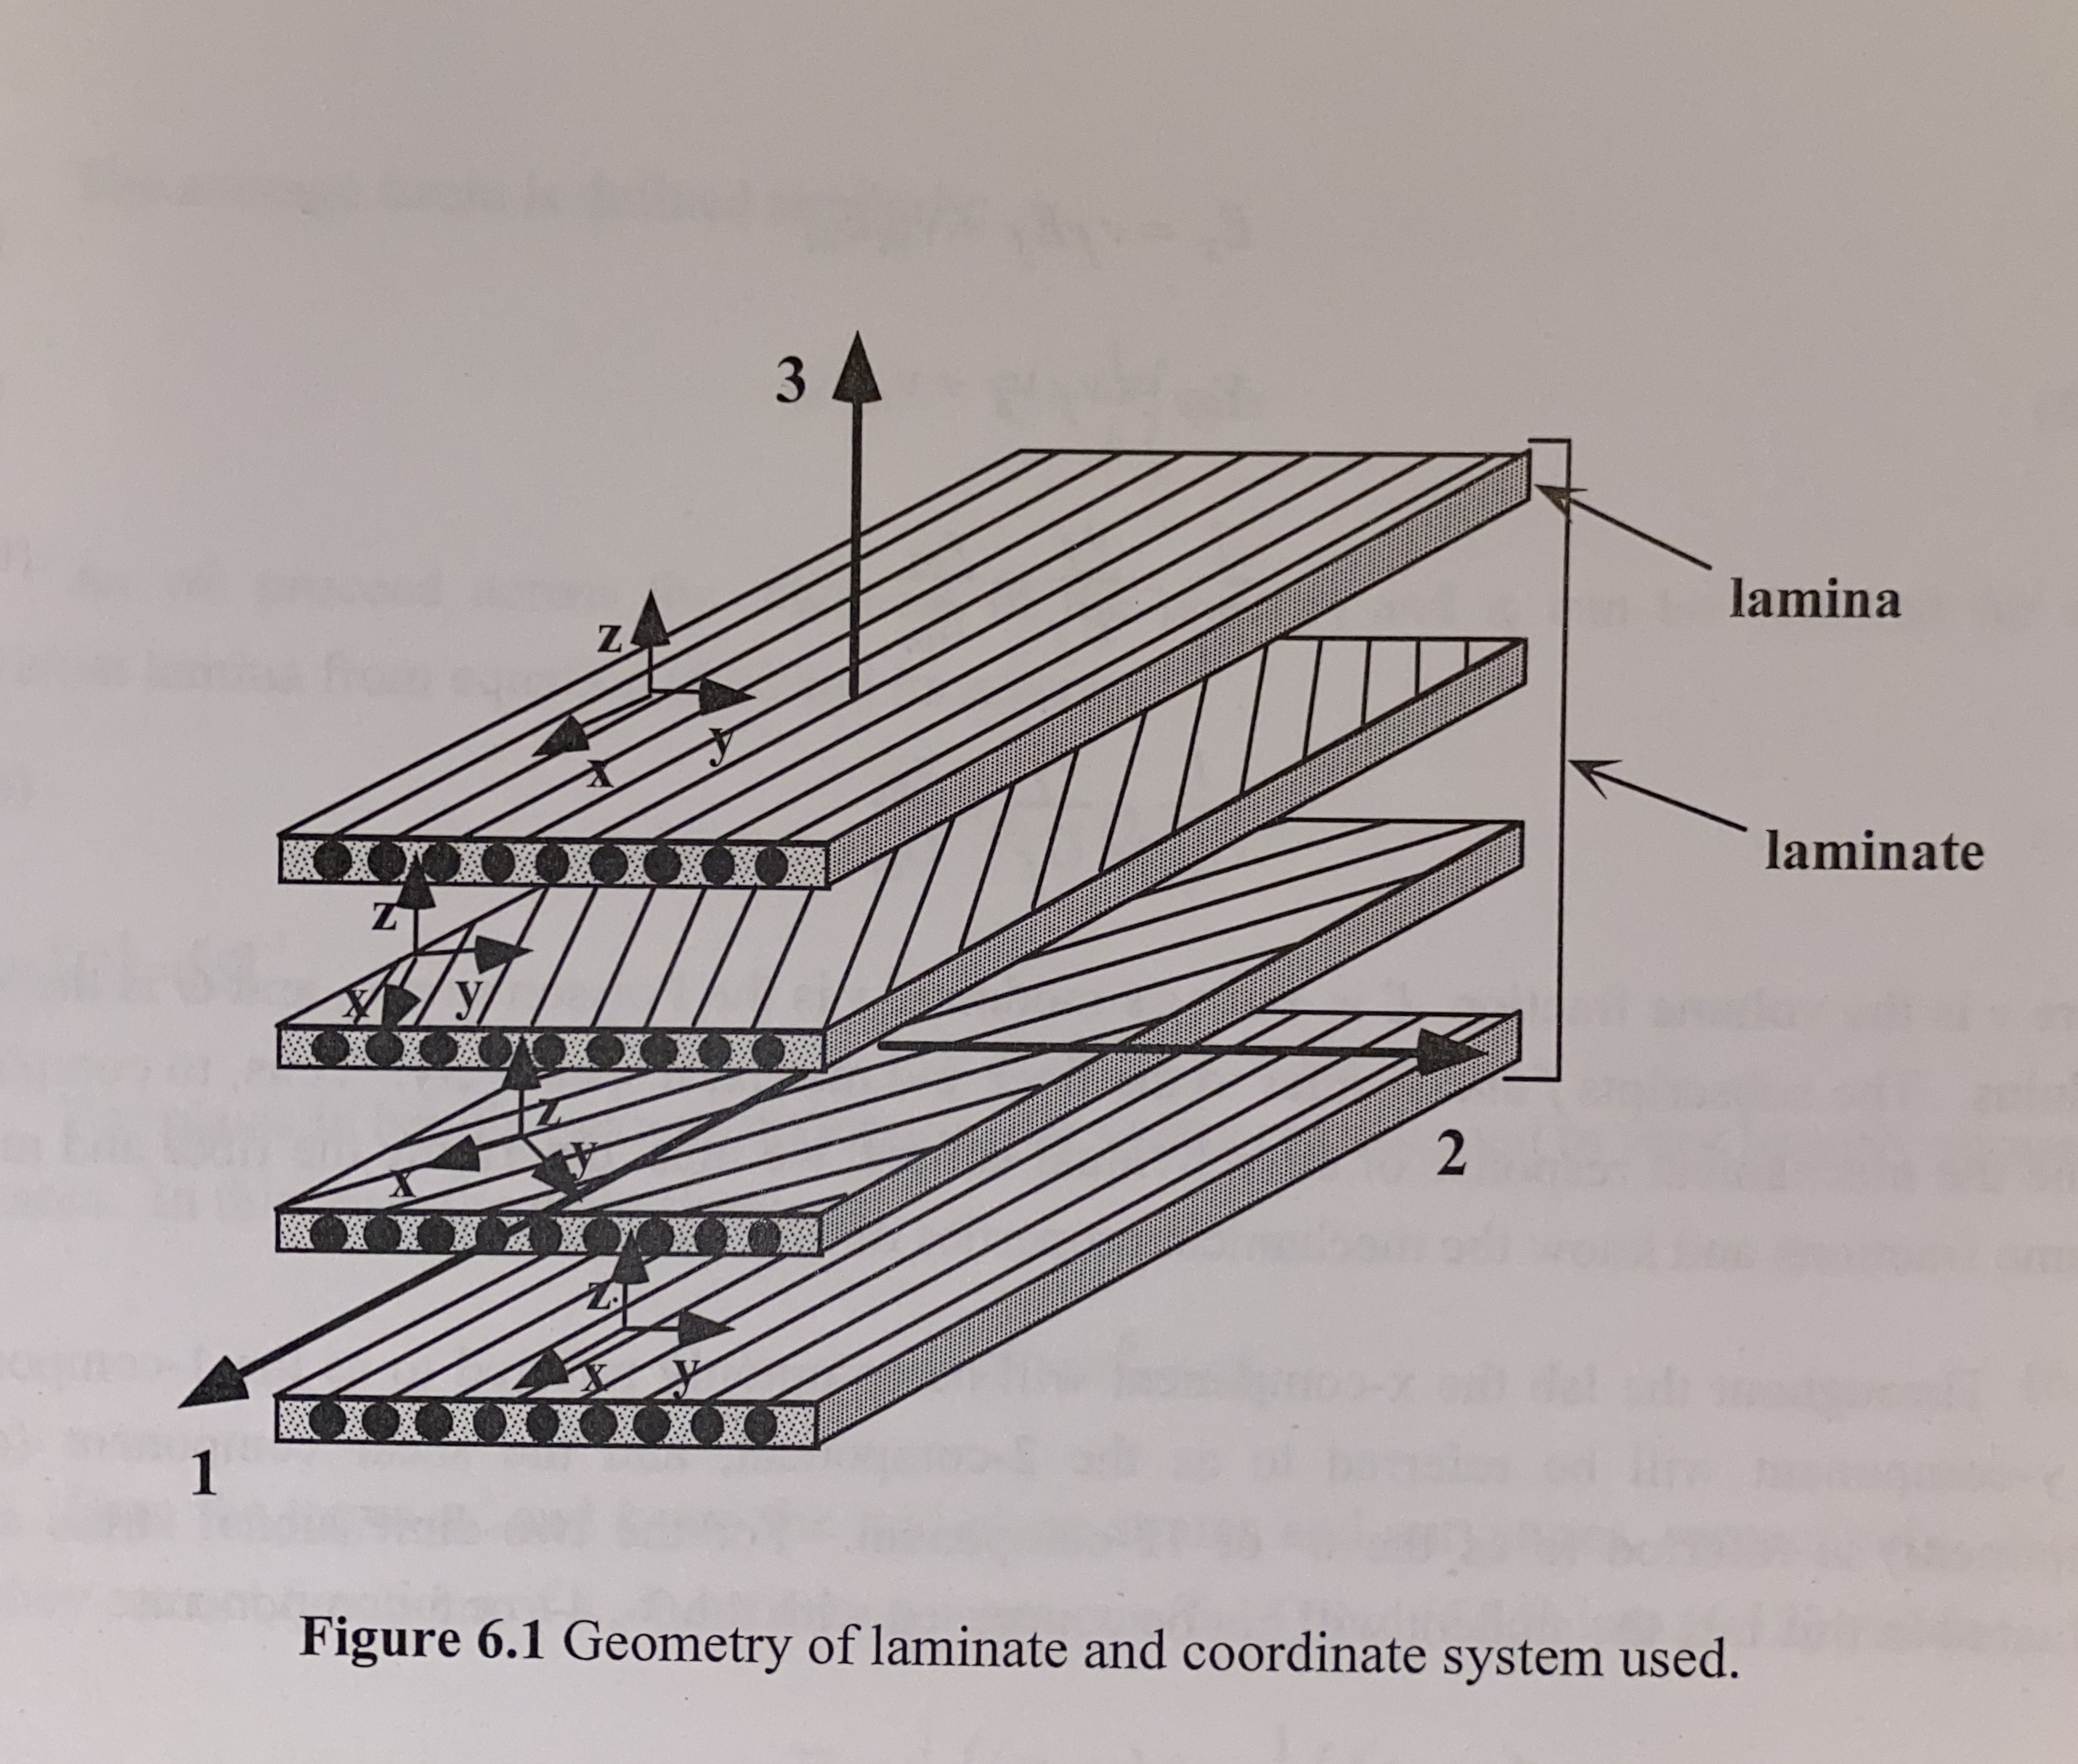
\includegraphics[width=0.45\textwidth]{Pictures/Theory and Analysis/coordsystem.jpg}
    \caption{Coordinate System\cite{labmanual}}
    \label{fig:coordsystem}
\end{figure}

Figure \ref{fig:coordsystem} shows the coordinate system used for analysis. Using this coordinate system and the assumption of plane stress, the only relevant stresses are $\sigma_1$ , $\sigma_2$, and $\sigma_6$. $\sigma_1$ and $\sigma_2$ correspond to the stresses in  x and y directions, while $\sigma_6$ corresponds to $xy$ shear stress. The stress-strain relationship is then:
\begin{equation}
    \epsilon_i = S_{ij}\sigma_j
\end{equation}
where $S_{ij}$ is the inverse of the previously mentioned stiffness matrix. For this case, we define $S_{ij}$ as:
\begin{equation}
    S_{ij} = 
    \begin{bmatrix}
    \frac{1}{E_x} & \frac{-\mbox{v}_{xy}}{E_x} & 0 \\
    \frac{-\mbox{v}_{xy}}{E_x} & \frac{1}{E_y} & 0 \\
    0 & 0 & \frac{1}{G_{xy}} 
    \end{bmatrix}
\end{equation}
where $E_x$ and $E_y$ are the longitudinal modulus and transverse modulus, $G_{xy}$ is the in-plane shear modulus, and v$_{xy}$ is the major Poisson's ratio. The stress-strain relationship for the lamina is now defined in terms of these constants. The values for these constants is estimated using the rule-of-mixtures (ROM). According to ROM, the constants can be calculated using the following equations.
\begin{equation}\label{eqn:eight}
    E_x = v_f E_f + v_mE_m
\end{equation}
\begin{equation} \label{eqn:nine}
    \mbox{v}_{xy} = v_f \mbox{v}_f + v_m \mbox{v}_m
\end{equation}
where $v$ is the volume fraction, $E$ represents Young's modulus, v represents Poisson's ratio, and G is the shear modulus. The stress-strain relationship for each lamina can now be calculated. Each individual lamina is stacked to form the laminate. It is then necessary to define the mechanical properties of the laminate in terms of the properties of each lamina layer. The laminates are modeled as plates, where the assumption of plane stress still holds. Thus, the relevant stresses are still $\sigma_1$, $\sigma_2$, and $\sigma_6$. The stress of the plate is then the average of the lamina stress values. 

\begin{equation}
    \overline{\sigma_{i}} = \frac{1}{h} \int_h \sigma_i dz
\end{equation}
Similarly for strain,

\begin{equation}
    \overline{\epsilon_{i}} = \frac{1}{h} \int_h \epsilon_i dz
\end{equation}
After evaluating the integration in these equations and substituting into the stress-strain relationship, the result is the following equation.

\begin{equation}
    \sigma_i = \frac{1}{h} A_{ij} \epsilon_{j}^{0} + \frac{1}{h} B_{ij} k_j
\end{equation}
where $A_{ij}$ is the laminate stiffness matrix and $B_{ij}$ is the coupling matrix.

\begin{equation}
    A_{ij} = \int_h Q_{ij}dz
\end{equation}
\begin{equation}
    B_{ij} = \int_h Q_{ij} z dz
\end{equation}
Because $Q_{ij}$ is constant woth respect ot the thickness of the ply, the expressions for $A_{ij}$ and $B_{ij}$ can be simplified.
\begin{equation}\label{eqn:15}
    A_{ij} = \sum_{k=1}^{N} (Q_{ij})_{k} (z_k - z_{k-1})
\end{equation}

\begin{equation}
    B_{ij} = \frac{1}{2} \sum_{k=1}^{N} (Q_{ij})_{k} (z_k^2 - z_{k-1}^2)
\end{equation}
Here, N is the number of plies and z is the distance from the midline to the $k^{th}$ ply. When a laminate is symmetric, the coupling matrix is eliminated. The resulting stress-strain relationship for a symmetric laminate is:
\begin{equation}
    \sigma_i = \frac{1}{h} A_{ij} \epsilon_{j}^{0}
\end{equation}

The in-plane stiffness matrix values are calculated using the following relationships:
\begin{equation} \label{eqn:18}
    \overline{Q}_{11} = cE_x
\end{equation}
\begin{equation}
    \overline{Q}_{22} = cE_y
\end{equation}
\begin{equation}
    \overline{Q}_{12} = c \mbox{v}_{xy} E_y
\end{equation}
\begin{equation}
    \overline{Q}_{66} = G_{xy}
\end{equation}
\begin{equation}\label{eqn:22}
    c = \left [1-\mbox{v}_{xy}^2 \frac{E_y}{E_x} \right]^{-1}
\end{equation}
Using the in-plane stiffness matrix, the off-axis stiffness matrix can be constructed.

After testing a composite laminate under uniaxial loading in a laboratory, the Young's modulus, shear modulus, and Poisson's ratio can be determined by analyzing the results. These constants can be predicted for comparison using the laminate stiffness matrix.
\begin{equation}
    E_1^0  = \frac{1}{a_{11}h}
\end{equation}
\begin{equation}
    E_2^0  = \frac{1}{a_{22}h}
\end{equation}
\begin{equation}
    \mbox{v}_{12}^0 = \frac{-a_{12}}{a_{11}}
\end{equation}
\begin{equation}
    G_6^0  = \frac{1}{a_{66}h}
\end{equation}
Note that a corresponds to the inverse of the laminate stiffness matrix ($A^{-1}$). 
\begin{comment}
Lastly, the failure properties of the material are considered. In this case, failure is defined using von Mises yield criterion. The yielding point occurs when distortion energy ($U_d$) reaches the following condition.

\begin{equation}
    U_d = \frac{1}{2G} J_2 = \frac{3}{4G} \tau_{oct}^2
\end{equation}
where $\tau_{oct}$ is the octahedral stress and $J_2$ is the second strain invariant. In the case of simple tension, $J_2$ for the yield point can be calculated as:

\begin{equation}
    J_2 = \frac{1}{3} \sigma^2
\end{equation}
\end{comment}
The von Misces and Tresca yield criterion are often used to investigate failure of isotropic materials, though analysis of failure of the composite laminate studied in this lab requires a more complicated approach. In this case, the quadratic polynomial failure theory is used. The primary equation used is:
\begin{equation}
    F_{ij} \sigma_{ij} \sigma_j + F_i \sigma_i = 1
\end{equation}
This equation defines the point at which failure will occur. $F_{ij}$ and $F_i$ are material parameters that characterize strength similarly to how yield strength corresponds to an isotropic material. The expressions to calculate these parameters are as follows:
\begin{equation}
    \overline{F}_{11} = \frac{1}{XX'}
\end{equation}
\begin{equation}
    \overline{F}_{22} = \frac{1}{YY'}
\end{equation}
\begin{equation}
    \overline{F}_{66} = \frac{1}{S^2}
\end{equation}
\begin{equation}
    \overline{F}_{12} = \frac{-1}{2}\sqrt{\overline{F}_{11} \overline{F}_{22}}
\end{equation}
\begin{equation}
    \overline{F}_{1} = \frac{1}{X} - \frac{1}{X'}
\end{equation}
\begin{equation}
    \overline{F}_{2} = \frac{1}{Y} - \frac{1}{Y'}
\end{equation}
Here, X and Y correspond to the longitudinal and transverse tension strength, while Y and Y' correspond to the longitudinal and transverse compression strength. S represents the in-plane shear stress. When considering the case of uniaxial tension, the quadratic polynomial failure equation becomes:

\begin{equation}
    F_{11} \sigma_{1}^2 + F_1 \sigma_1 = 1
\end{equation}







